%%
%% This is file `sample-sigconf-authordraft.tex',
%% generated with the docstrip utility.
%%
%% The original source files were:
%%
%% samples.dtx  (with options: `all,proceedings,bibtex,authordraft')
%% 
%% IMPORTANT NOTICE:
%% 
%% For the copyright see the source file.
%% 
%% Any modified versions of this file must be renamed
%% with new filenames distinct from sample-sigconf-authordraft.tex.
%% 
%% For distribution of the original source see the terms
%% for copying and modification in the file samples.dtx.
%% 
%% This generated file may be distributed as long as the
%% original source files, as listed above, are part of the
%% same distribution. (The sources need not necessarily be
%% in the same archive or directory.)
%%
%%
%% Commands for TeXCount
%TC:macro \cite [option:text,text]
%TC:macro \citep [option:text,text]
%TC:macro \citet [option:text,text]
%TC:envir table 0 1
%TC:envir table* 0 1
%TC:envir tabular [ignore] word
%TC:envir displaymath 0 word
%TC:envir math 0 word
%TC:envir comment 0 0
%%
%% The first command in your LaTeX source must be the \documentclass
%% command.
%%
%% For submission and review of your manuscript please change the
%% command to \documentclass[manuscript, screen, review]{acmart}.
%%
%% When submitting camera ready or to TAPS, please change the command
%% to \documentclass[sigconf]{acmart} or whichever template is required
%% for your publication.
%%
%%
\documentclass[acmtog]{acmart}
%%
%% \BibTeX command to typeset BibTeX logo in the docs
\AtBeginDocument{%
  \providecommand\BibTeX{{%
    Bib\TeX}}}

\usepackage{multirow}
\usepackage{enumitem}

%% Rights management information.  This information is sent to you
%% when you complete the rights form.  These commands have SAMPLE
%% values in them; it is your responsibility as an author to replace
%% the commands and values with those provided to you when you
%% complete the rights form.


\copyrightyear{2025}
\acmYear{2025}
\setcopyright{acmlicensed}\acmConference[SA Conference Papers '25]{SIGGRAPH Asia 2025 Conference Papers}{December 15--18, 2025}{Hong Kong, Hong Kong}
\acmBooktitle{SIGGRAPH Asia 2025 Conference Papers (SA Conference Papers '25), December 15--18, 2025, Hong Kong, Hong Kong}
\acmDOI{10.1145/3757377.3763951}
\acmISBN{979-8-4007-2137-3/2025/12}
%%
%% Submission ID.
%% Use this when submitting an article to a sponsored event. You'll
%% receive a unique submission ID from the organizers
%% of the event, and this ID should be used as the parameter to this command.
\acmSubmissionID{1949}

%%
%% For managing citations, it is recommended to use bibliography
%% files in BibTeX format.
%%
%% You can then either use BibTeX with the ACM-Reference-Format style,
%% or BibLaTeX with the acmnumeric or acmauthoryear sytles, that include
%% support for advanced citation of software artefact from the
%% biblatex-software package, also separately available on CTAN.
%%
%% Look at the sample-*-biblatex.tex files for templates showcasing
%% the biblatex styles.
%%

%%
%% The majority of ACM publications use numbered citations and
%% references.  The command \citestyle{authoryear} switches to the
%% "author year" style.
%%
%% If you are preparing content for an event
%% sponsored by ACM SIGGRAPH, you must use the "author year" style of
%% citations and references.
%% Uncommenting
%% the next command will enable that style.
\citestyle{acmauthoryear}


%%
%% end of the preamble, start of the body of the document source.
\begin{document}

%%
%% The "title" command has an optional parameter,
%% allowing the author to define a "short title" to be used in page headers.
\title{PhysHMR: Learning Humanoid Control Policies from Vision for Physically Plausible Human Motion Reconstruction}

%%
%% The "author" command and its associated commands are used to define
%% the authors and their affiliations.
%% Of note is the shared affiliation of the first two authors, and the
%% "authornote" and "authornotemark" commands
%% used to denote shared contribution to the research.
\author{Qiao Feng}
\email{fengqiao@seas.upenn.edu}
\orcid{0000-0003-0625-651X}
\affiliation{%
  \institution{University of Pennsylvania}
  \city{Philadelphia}
  \state{Pennsylvania}
  \country{USA}
}

\author{Yiming Huang}
\email{ymhuang9@seas.upenn.edu}
\orcid{0009-0004-4001-0630}
\affiliation{%
  \institution{University of Pennsylvania}
  \city{Philadelphia}
  \state{Pennsylvania}
  \country{USA}
}


\author{Yufu Wang}
\email{yufu@seas.upenn.edu}
\orcid{0000-0001-9907-8382}
\affiliation{%
  \institution{University of Pennsylvania}
  \city{Philadelphia}
  \state{Pennsylvania}
  \country{USA}
}

\author{Jiatao Gu}
\email{jgu32@cis.upenn.edu}
\orcid{0000-0003-3578-2711}
\affiliation{%
  \institution{University of Pennsylvania}
  \city{Philadelphia}
  \state{Pennsylvania}
  \country{USA}
}

\author{Lingjie Liu}
\email{lingjie.liu@seas.upenn.edu}
\orcid{0000-0003-4301-1474}
\affiliation{%
  \institution{University of Pennsylvania}
  \city{Philadelphia}
  \state{Pennsylvania}
  \country{USA}
}


%%
%% By default, the full list of authors will be used in the page
%% headers. Often, this list is too long, and will overlap
%% other information printed in the page headers. This command allows
%% the author to define a more concise list
%% of authors' names for this purpose.
\renewcommand{\shortauthors}{Qiao et al.}

%%
%% The abstract is a short summary of the work to be presented in the
%% article.
\begin{abstract}
Reconstructing physically plausible human motion from monocular videos remains a challenging problem in computer vision and graphics. Existing methods primarily focus on kinematics-based pose estimation, often leading to unrealistic results due to the lack of physical constraints. To address such artifacts, prior methods have typically relied on physics-based post-processing following the initial kinematics-based motion estimation. However, this two-stage design introduces error accumulation, ultimately limiting the overall reconstruction quality.
In this paper, we present PhysHMR, a unified framework that directly learns a visual-to-action policy for humanoid control in a physics-based simulator, enabling motion reconstruction that is both physically grounded and visually aligned with the input video. A key component of our approach is the pixel-as-ray strategy, which lifts 2D keypoints into 3D spatial rays and transforms them into global space.
These rays are incorporated as policy inputs, providing robust global pose guidance without depending on noisy 3D root predictions. This soft global grounding, combined with local visual features from a pretrained encoder, allows the policy to reason over both detailed pose and global positioning. To overcome the sample inefficiency of reinforcement learning, we further introduce a distillation scheme that transfers motion knowledge from a mocap-trained expert to the vision-conditioned policy, which is then refined using physically motivated reinforcement learning rewards. Extensive experiments demonstrate that PhysHMR produces high-fidelity, physically plausible motion across diverse scenarios, outperforming prior approaches in both visual accuracy and physical realism.
\end{abstract}




%%
%% The code below is generated by the tool at http://dl.acm.org/ccs.cfm.
%% Please copy and paste the code instead of the example below.
%%
\begin{CCSXML}
<ccs2012>
   <concept>
       <concept_id>10010147.10010257</concept_id>
       <concept_desc>Computing methodologies~Machine learning</concept_desc>
       <concept_significance>500</concept_significance>
       </concept>
   <concept>
       <concept_id>10010147.10010371.10010352</concept_id>
       <concept_desc>Computing methodologies~Animation</concept_desc>
       <concept_significance>500</concept_significance>
       </concept>
 </ccs2012>
\end{CCSXML}

\ccsdesc[500]{Computing methodologies~Machine learning}
\ccsdesc[500]{Computing methodologies~Animation}

%%
%% Keywords. The author(s) should pick words that accurately describe
%% the work being presented. Separate the keywords with commas.
\keywords{Motion reconstruction, Physical plausibility, Humanoid control, Monocular video}
%% A "teaser" image appears between the author and affiliation
%% information and the body of the document, and typically spans the
%% page.
\begin{teaserfigure}
\centering
\includegraphics[width=\textwidth]{Figs/teaser.pdf}
\caption{
Given a monocular video (a), (b) kinematic-based methods (e.g., GVHMR~\cite{shen2024gvhmr}) often cannot produce physically plausible results and suffer from artifacts like foot floating. (c) While tracking-based controllers (e.g., PHC+~\cite{Luo2023PerpetualHC}) can enforce physical plausibility, they may amplify errors from inaccurate motion reconstruction, leading to unnatural behaviors. (d) In contrast, our PhysHMR model learns a visual-to-action policy that directly predicts control signals from visual input, preventing error amplification and producing motions that are both physically plausible and visually aligned with the input video (a). As videos are the most effective way to assess the physical plausibility of the results, we encourage readers to view our supplementary video. 
}
  \Description{teaser}
  \label{fig:teaser}
\end{teaserfigure}

%%  \received{20 February 2007}
%%  \received[revised]{12 March 2009}
%%  \received[accepted]{5 June 2009}

%%
%% This command processes the author and affiliation and title
%% information and builds the first part of the formatted document.
\maketitle
\section{Introduction}

Recently, agent systems based on Large Language Models (LLMs) have attracted significant research interest. With the rapid development of AI technologies, LLM-based agent systems dynamically handle complex tasks in various interactive environments, alleviating human burdens. Agent systems are increasingly applied across diverse fields~\citep{liu2025advances}, including clinical treatment~\citep{wang2025surveyllmbasedagentsmedicine}, scientific simulations~\citep{park2023generativeagentsinteractivesimulacra}, and software engineering~\citep{wang2025openhandsopenplatformai}.

Despite the considerable attention agent systems have received, their security remains an urgent area for improvement~\citep{wang2025comprehensivesurvey,yu2025asurveytrustagent}. One security topic previously discussed in cybersecurity yet still crucial in agent systems, is \textbf{access control (AC)}. To minimize the loss caused by privilege escalation or unexpected behavior, systems require optimal permission allocation strategies that are adapted to the generative behavior patterns of LLM-based agents. Traditional AC models, built on static rules and binary allow/deny logic~\citep{ferraiolo2009rolebasedaccesscontrols,8594462}. Early research proposed formal methods based on Information Flow Control (IFC)~\citep{myers1997decentralized} to allocate permissions, ensuring secure interactions among system entities. Subsequent advances extended these mechanisms to incorporate contextual factors such as user role, location, and time
~\citep{covington2001context}. Unfortunately, traditional IFC mechanisms face severe limitations in handling dynamic, implicit semantics or complex interactive behaviors, which renders agent access control vulnerable. Our vision paper underscores the importance of access control in agent systems, and argues that strategies for permission allocation must \textbf{move beyond the traditional focus on securing static data, to instead emphasize the governance of dynamic information flow.} Therefore, we envision \textbf{Agent Access Control (AAC)} as a novel framework which redefines access control not as an external security gate, but as an intrinsic cognitive capability of the agent itself. The core of AAC is to view information disclosure as a process of judging appropriateness based on reasoning and context, rather than relying only on fixed rules.

To realize this vision, our AAC framework is built upon two integrated modules, executed by a dedicated reasoning engine: (1) Multi-dimensional Contextual Evaluation, which analyzes the holistic context of an interaction, and (2) Adaptive Response Formulation, which crafts nuanced, appropriate information outputs. In the following content, we begin by detailing the framework, then explore the critical role of its core reasoning engine for effective access control. Finally, the future implications and challenges of this new paradigm will be presented to pave the way for agents that are not only capable, but trustworthy.


\section{Related Work}
\label{sec:related}

\sssection{Image-to-video Generation.} Visual content generation and editing have witnessed significant advancements thanks to the emergence of diffusion models~\citep{ddpm, ddim, ldm}. Recently, DiT~\citep{dit} has become the mainstream architecture of the denoising model with promising generation quality, surpassing U-Net~\citep{unet} with its powerful scaling capability~\citep{kaplan2020scalinglawsneurallanguage} and potential for multimodal interaction~\citep{sd3}. Flow Matching~\citep{flowmatching, rectifiedflow} introduces an improved generative model paradigm that interpolates data and noise linearly in the forward diffusion process, bringing better theoretical properties and conceptual simplicity. Building upon these works, a number of I2V models~\citep{wan, easyanimate, hunyuanvideo, cogvideox, opensora2, vchitect2} have emerged with full 3D attention~\citep{attention2017} instead of decoupled spatiotemporal attention~\citep{guo2024animatediff}, significantly enhancing generation quality and consistency.

% Image-conditioned video editing methods leverage the temporal prior of I2V models to propagate the edited keyframe along the temporal dimension while preserving structure and motion consistency with the source video. Videoshop~\citep{videoshop} introduces noise extrapolation to enhance the inversion process. DreamMotion~\citep{dreammotion} utilizes score distillation sampling (SDS)~\citep{pooledreamfusion} to optimize the source video latents towards the condition image, during which space-time self-similarities constraints are applied to better match the source video. I2VEdit~\citep{i2vedit} first trains a sample-specific motion LoRA~\citep{lora} and then performs attention matching between the EDM~\citep{edm} inversion and denoising process. AnyV2V~\citep{kuanyv2v} performs DDIM~\citep{ddim} inversion and exploits an attention injection paradigm to ensure consistency with the source video. VideoRepainter~\citep{videorepainter} repurposes an I2V model for editing by fine-tuning it with a symmetric condition mechanism to avoid mask ambiguity caused by downsampling. VACE~\citep{vace} provides an all-in-one solution for video editing by introducing a ControlNet-style~\citep{controlnet} Context Adapter structure, which requires extensive training. These approaches include either model-specific designs or costly optimization, limiting their ability to keep up with the rapid advancement of I2V models.

\sssection{Training-free Visual Editing.} Training-free visual editing modifies the source image or video according to designated conditions (e.g., text, image, and mask) at test time, using off-the-shelf pretrained models. Existing works can be broadly categorized into two categories: inversion-based and optimization-based methods. Inversion-based methods~\citep{videoshop, dni, wave, yatim2025dynvfxaugmentingrealvideos} adopt the inversion of the diffusion process to map the input back to Gaussian noise, and then perform denoising under given conditions. However, not only is the inversion process time-consuming, but it also inevitably induces error. To overcome the inherent inaccuracy of inversion and ensure consistency with the input, various attention injection strategies~\citep{wave, yatim2025dynvfxaugmentingrealvideos} are utilized to further incorporate source information. Despite their effectiveness, these strategies are model-specific, reducing their universality to different model structures. Optimization-based methods~\citep{dreammotion, ren2025fdsfrequencyawaredenoisingscore, unityindiversity} use SDS~\citep{pooledreamfusion} to directly optimize the input latents towards the desired direction. Nevertheless, the optimization operation introduces considerable computational cost, limiting its availability to common creators. With the prevalence of flow-based models~\citep{flowmatching, rectifiedflow}, there have also been methods~\citep{avrahami2025stableflowvitallayers, dalva2024fluxspacedisentangledsemanticediting, xu2025unveilinversioninvarianceflow} that leverage the properties of the flow matching process to achieve more precise and consistent visual editing. However, few solutions are both lightweight and universal without model-specific design in the video domain, limiting creators to swiftly leverage the most up-to-date I2V base models for video editing within user-friendly resources, such as a single GPU.
% to take the temporal dimension into account.

There have also been works exploring inversion-free image editing. For instance, InfEdit~\citep{infedit} theoretically depends on the diffusion process, limiting its application to state-of-the-art flow-based models. It also needs attention manipulation, further limiting its universality. FlowEdit~\citep{kulikov2024floweditinversionfreetextbasedediting} leverages flow properties to construct a transport from the source to the target distribution, which is derived from the Euler Discrete Solver~\citep{sd3}. In contrast, our method constructs two parallel ODEs to model the editing process, which does not depend on a specific ODE solver and enables control over editing strength. Our method also introduces SMPI to further enhance video-level spatiotemporal consistency and a flexible caching strategy.

\section{Method}
%
Next, we formulate the target task and describe the training data generation and representation learning. 
An overview of the proposed generation process is shown in \cref{fig:overview}.

\subsection{Task formulation}
%
The target task is instance-level image retrieval.
Given a query image, the goal is to retrieve all positive images from a database (db), \ie those that depict the same object instance as the query.
Images depicting different object instances, even if they belong to the same semantic category, are negatives and should not be retrieved.
This is an open-world task, testing on unseen objects from a variety of domains which may be seen or unseen during training.

We consider the efficient retrieval variant using global descriptors.  
Formally, an image $x$ is mapped to a $d$-dimensional global descriptor $\mathbf{z} = f_\theta(x) \in \mathbb{R}^d$.  
Retrieval is performed via nearest neighbor search in Euclidean space, ranking database descriptors based on their cosine similarity to the query.  
The encoder, parameterized by $\theta$, is optimized during training.
We focus on fine-tuning foundational models~\citep{zhai2023sigmoid} that already perform well by pretraining.  

\begin{figure*}[t]
% \vspace{5pt}
\centering
\includegraphics[width=.95\linewidth]{fig/overview.pdf}
% \vspace{-5pt}
\caption{Overview of instance-level training data generation.
A domain name or description is the only input, which is used to prompt an LLM to provide a list of object category names. 
Then, we generate examples of those categories using a GDM, remove the background, and synthesize lighting and background multiple times per generated example to create a diverse set of positive images for each instance.
} 
\label{fig:overview}
\end{figure*}

\subsection{Instance-level training data generation}
%
We propose a pipeline that requires only the name, or a textual description, of a target domain as input, and automatically generates an image training set with instance-level labels.
The process consists of four stages:
(i) \textit{Objects categories generation} by prompting an LLM to provide a list of %useful 
object category names;
(ii) \textit{Object instance generation} by prompting a GDM to generate object instances from each category;
(iii) \textit{Background generation} by synthesizing diverse backgrounds per instance;
(iv) \textit{Viewpoint variations} by augmenting the generated images with geometric transformations.
Each stage of the process is detailed below.

\paragraph{Object categories generation}
%
Object categories (\eg \textit{table}, \textit{chair}, \textit{clock}) are needed to prompt the GDM for image generation. 
We automatically obtain a list of object categories by prompting an LLM with minimal information about the domain of interest. 
In the general case in which we do not target a specific domain, the prompt we use is 
``\emph{Provide a raw list of names of everyday objects.}''
For specific domains, such as artwork, landmark, or product, we enrich the prompt with relevant information and hint with a few examples of object categories. 
Full details of the designed prompts are provided in the supplementary material. 
This approach yields a rich and diverse list of $C$ object categories.
Examples of category names generated for the general case are \textit{sofa}, \textit{desk}, while for the specific domains are \textit{bust}, \textit{castle}, and \textit{polaroid film}, for artwork, landmark, and product, respectively.

\paragraph{Object instance generation}
%
We prompt a GDM, in particular Stable Diffusion Turbo~\citep{sauer2025adversarial}, with an object category to generate $K$ images per category.
We assume that generating images with different random seeds produces variations that are distinct and recognizable as separate instances within the same category. 
Therefore, following an instance-level class definition, each of the $M$ generated images, where $M = C K$, is treated as a separate class in our training set.
To facilitate the follow-up step of background generation, we target a simple or uniform background. To achieve this, we add ``\emph{in a clean background}" to the prompt after the object category as in, ``\textit{a table in a clean background}." 
%
Examples in \cref{fig:sdimages} show that, even though the background removal process may fail in both cases, it is less likely to happen with the extended prompt, while the original prompt provides outputs with richer background.


\begin{figure*}[t]
\begin{center}    
% \vspace{5pt}
\footnotesize
\newcommand{\figclean}[2]{\includegraphics[width=42pt,height=42pt]{fig/sd/#1/clean/#2.png}&\includegraphics[width=42pt,height=42pt]{fig/sd/#1/clean/#2_fg.png}}
\newcommand{\figunclean}[2]{\includegraphics[width=42pt,height=42pt]{fig/sd/#1/unclean/#2.png}&\includegraphics[width=42pt,height=42pt]{fig/sd/#1/unclean/#2_fg.png}}
% \begin{tabular}{lcccccccc}
%                                         & sofa & sofa & lamp & X & X & X & X & X \\
% \raisebox{15pt}{SD - clean}  			& \includegraphics[width=42pt,height=42pt]{fig/sd/clean/sofa/0.png}					& \includegraphics[width=42pt,height=42pt]{fig/sd/clean/sofa/7.png} 			& \includegraphics[width=42pt,height=42pt]{fig/sd/clean/lamp/8.png} 			& \includegraphics[width=42pt,height=42pt]{fig/sd/clean/lamp/8.png} 				& \includegraphics[width=42pt,height=42pt]{fig/sd/clean/lamp/8.png} 		   & \includegraphics[width=42pt,height=42pt]{fig/sd/clean/lamp/8.png} 				  & \includegraphics[width=42pt,height=42pt]{fig/sd/clean/lamp/8.png} 		     & \includegraphics[width=42pt,height=42pt]{fig/sd/clean/lamp/8.png} 				 \\
% \raisebox{15pt}{bg. removal}           	& \includegraphics[width=42pt,height=42pt]{fig/sd/clean/sofa_rmv/fg_00360.png}  	& \includegraphics[width=42pt,height=42pt]{fig/sd/clean/sofa_rmv/fg_00388.png}  & \includegraphics[width=42pt,height=42pt]{fig/sd/clean/lamp_rmv/fg_32112.png}  & \includegraphics[width=42pt,height=42pt]{fig/sd/clean/lamp_rmv/fg_32112.png} 		& \includegraphics[width=42pt,height=42pt]{fig/sd/clean/lamp_rmv/fg_32112.png} & \includegraphics[width=42pt,height=42pt]{fig/sd/clean/lamp_rmv/fg_32112.png}  	  & \includegraphics[width=42pt,height=42pt]{fig/sd/clean/lamp_rmv/fg_32112.png} & \includegraphics[width=42pt,height=42pt]{fig/sd/clean/lamp_rmv/fg_32112.png}  	 \\
% \raisebox{15pt}{SD - not clean}      	& \includegraphics[width=42pt,height=42pt]{fig/sd/noclean/sofa/1.png}				& \includegraphics[width=42pt,height=42pt]{fig/sd/noclean/sofa/1.png}           & \includegraphics[width=42pt,height=42pt]{fig/sd/noclean/lamp/8.png} 			& \includegraphics[width=42pt,height=42pt]{fig/sd/noclean/lamp/8.png}  				& \includegraphics[width=42pt,height=42pt]{fig/sd/noclean/lamp/8.png} 		   & \includegraphics[width=42pt,height=42pt]{fig/sd/noclean/lamp/8.png}   		      & \includegraphics[width=42pt,height=42pt]{fig/sd/noclean/lamp/8.png} 		 & \includegraphics[width=42pt,height=42pt]{fig/sd/noclean/lamp/8.png}   		     \\
% \raisebox{15pt}{bg. removal}  	        & \includegraphics[width=42pt,height=42pt]{fig/sd/noclean/sofa/1.png}  				& \includegraphics[width=42pt,height=42pt]{fig/sd/noclean/sofa/7.png}           & \includegraphics[width=42pt,height=42pt]{fig/sd/noclean/lamp/8.png} 			& \includegraphics[width=42pt,height=42pt]{fig/sd/noclean/lamp/8.png} 				& \includegraphics[width=42pt,height=42pt]{fig/sd/noclean/lamp/8.png}          & \includegraphics[width=42pt,height=42pt]{fig/sd/noclean/lamp/8.png}  	          & \includegraphics[width=42pt,height=42pt]{fig/sd/noclean/lamp/8.png}          & \includegraphics[width=42pt,height=42pt]{fig/sd/noclean/lamp/8.png}  	         \\
% \end{tabular}
\begin{tabular}{@{\hspace{0pt}}r@{\hspace{2pt}}c@{\hspace{2pt}}c@{\hspace{2pt}}c@{\hspace{2pt}}cr@{\hspace{2pt}}c@{\hspace{2pt}}c@{\hspace{2pt}}c@{\hspace{2pt}}c@{\hspace{0pt}}}
\raisebox{15pt}{bicycle} & \figclean{Bicycles}{sd_clean_Bicycles_2} & \figunclean{Bicycles}{sd_unclean_Bicycles_1} &\raisebox{15pt}{headphones} & \figclean{headphones}{sd_clean_headphones_1} & \figunclean{headphones}{sd_unclean_headphones_3}\\[5pt]
\raisebox{15pt}{luggage} & \figclean{luggage}{sd_clean_luggage_2} & \figunclean{luggage}{sd_unclean_luggage_0} & \raisebox{15pt}{women's jumpsuit} & \figclean{Womens-jumpsuit}{sd_clean_Womensjumpsuit_0} & \figunclean{Womens-jumpsuit}{sd_unclean_Womensjumpsuit_0}\\[5pt]
\raisebox{15pt}{temple} & \figclean{Temple}{sd_clean_Temple_0} & \figunclean{Temple}{sd_unclean_Temple_2} & \raisebox{15pt}{juicing machine} & \figclean{Juicing-machine}{sd_clean_Juicingmachine_4} & \figunclean{Juicing-machine}{sd_unclean_Juicingmachine_0}\\[5pt]
\raisebox{15pt}{toy car} & \figclean{toy-car}{sd_clean_toycar_1} & \figunclean{toy-car}{sd_unclean_toycar_1} &
\raisebox{15pt}{French empire clock} & \figclean{French-Empire-clock}{sd_clean_FrenchEmpireclock_1} & \figunclean{French-Empire-clock}{sd_unclean_FrenchEmpireclock_0}
\end{tabular}
% \vspace{5pt}
\caption{Examples of object instances generated by GDM for specific categories. We show the category name, the generated image and the background removal process with using ``\emph{in a clean background}'' (columns 1 \& 2) and without it (columns 3 \& 4).\label{fig:sdimages}}
\end{center}
\end{figure*}





\paragraph{Background generation} We create variations of an object instance by generating images with multiple, distinct backgrounds and lighting conditions. Given a generated instance in the previous step, we rely on ICLight \citep{iclight} to perform the relighting and add different backgrounds. Firstly, background removal is conducted to ensure that the input image only depicts the object of interest. 
Our generated images are typically quite easy to have their background removed. We additionally perform padding with a random amount and resize to the original resolution so that the object appears at different sizes and positions. Then, the object category is used as a prompt, which guides ICLight to generate an environment that is commonly appropriate for the specific object.
We repeat this process $N$ times per generated object instance with different seeds to generate multiple backgrounds. 
The $N$ images are all elements of the same class in our training set and the only members of this class.
\cref{fig:iclight} shows examples of generated lighting and background for a variety of object categories.

\paragraph{Viewpoint variations}
%
All images of a class depict the object under different background and  similar viewpoint which only varies because of the padding of the previous step. We additionally rely on simple random geometric augmentations during training to further modify the object's geometry. 
This process resembles self-supervised learning with instance-discrimination~\citep{odm+23,chen2020simple}, where two positive examples are just two different random augmentations of the same input image. 
Nevertheless, there is an essential difference in our case, that the background and lighting significantly vary. Such a factor makes our training setting a unique of its kind.

\begin{figure*}[!h]
\centering
\hspace{-0.9cm}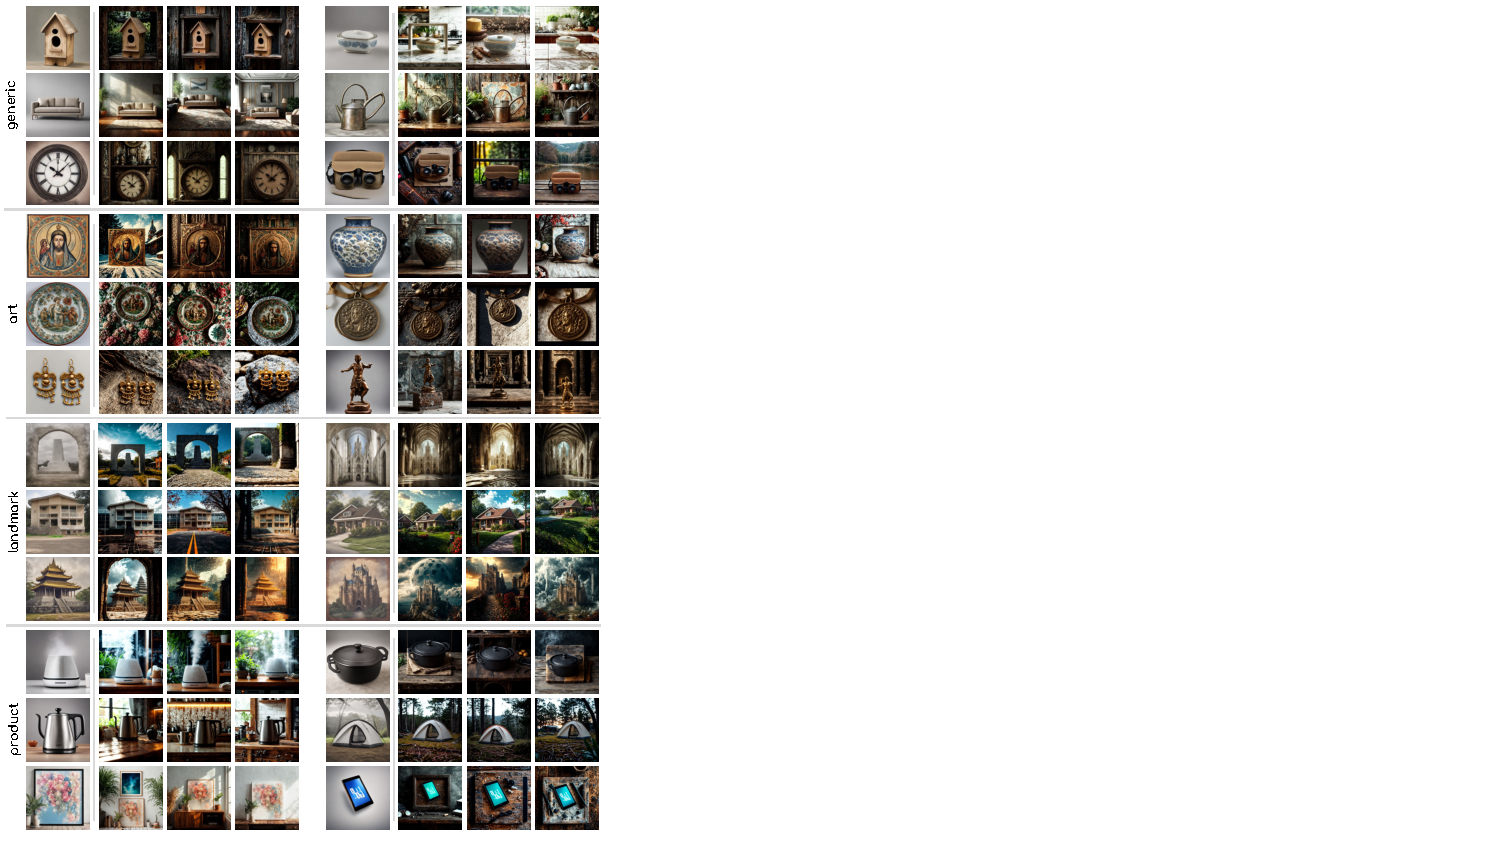
\includegraphics[width=0.91\linewidth]{fig/example.pdf}
\vspace{-9pt}
\caption{Examples of object instances generated by GDM (column 1), and the generated images that leave the object intact and add lighting and background that is well suited to the object (columns 2 $\sim$ 4).
\label{fig:iclight}}
\end{figure*}

\subsection{Representation learning}
%
In total, our generated dataset contains $CKN$ training images, forming $CK$ classes coming from $C$ object categories. 
We construct training batches by sampling $B$ classes and all their corresponding images, resulting in $NB$  images per batch. 
During training, we adopt a query \vs database scheme:
one image from each of the $N$ images per class is randomly chosen as the query, while the remaining $NB-1$ images of the batch form the database, as shown in \cref{fig:batch}.

The similarity between the query and db images is computed in $\hat{\mathbf{y}} \in \mathbb{R}^{NB-1}$, while $\mathbf{y} \in \{0,1\}^{NB-1}$ denotes the labels of all db images with respect to the query, \ie positive or negatives based on their classes. 
We optimize an information retrieval metric as the loss function, in particular an approximation of recall at the top-$k$ ranks, based on $\hat{\mathbf{y}}$, and $\mathbf{y}$.
We train with the average of recall@k loss estimated for different values of $k$.
The approximation of recall is possible by formulating its estimation with the use of step functions, which, during training, are replaced with a sigmoid function.
The technical and implementation details can be found in the original paper~\citep{ptm22}.





\begin{figure}[t]
\begin{center}
\includegraphics[width=0.83\linewidth]{fig/batch.pdf}
\vspace{-10pt}
\caption{Training batch construction for instance-level representation learning. A batch simulates a retrieval task with a query (blue) and database of positive (green) and negative (red) images. Images are considered positive if they belong to the same class, otherwise they are negatives. An image encoder is trained with metric learning on this batch.}
\label{fig:batch}
\end{center}
\end{figure}

\begin{table}[t]
    \centering
    \caption{Statistics of the generated training dataset. \oursgeneric{} and \oursspecific{} comprise only objects from the generic domain and one of the specific domains, respectively.  
    \oursplus{} comprises 50\% of objects from the generic domain ($10$K) and all objects from the three specific domains ($10$K), \ie $20$K objects in total.}
\small
\begin{tabular}{lrrr}
\toprule
\textbf{domain of objects}  & $C$ & $K$ & \textbf{instances} \\ 
\midrule
generic           & $2,000$  & $10$ & $20,000$ \\ 
art        & $200$  & $15$ & $3,000$ \\ 
landmark   & $50$ & $80$  & $4,000$ \\
product    & $200$ & $15$  & $3,000$ \\  
\bottomrule
\end{tabular}

\label{tab:gene_details}
\end{table}



\section{Experiments}
\begin{figure*}[t]
    \centering
    \includegraphics[width=0.98\linewidth]{Figs/main.pdf}
\caption{
Comparison against two physics-based methods. The black line indicates the ground. PhysPT (row 2) uses neural networks to approximate physics, but still suffers from ground penetration. PHC+ (row 3) amplifies motion reconstruction errors during tracking, leading to unstable results. Both methods cannot correct upstream errors. In contrast, our visual-to-action approach produces motion that is both physically plausible and visually aligned.
}
  \Description{Comparison}
    \label{results}
\end{figure*}

\begin{table*}[t]
\centering
\caption{Comparison of our motion reconstruction variants on AIST++ and EMDB2 under kinematic and physical plausibility metrics. Lower is better.}
\label{tab:main}
\small
\begin{tabular}{l l 
                c c c c c c c 
                c c c c c c c}
\toprule
\multirow{2}{*}{{Phys. Type}} & \multirow{2}{*}{{Method}} 
& \multicolumn{7}{c}{{EMDB2}} 
& \multicolumn{7}{c}{{AIST++}} \\
\cmidrule(lr){3-9} \cmidrule(lr){10-16}
 &  & PA & WA & MPJ & FS & HV & ACC & VEL
     & PA & WA & MPJ & FS & HV & ACC & VEL \\
\midrule
\multirow{2}{*}{Kin.} 
    & TRAM               &  \textbf{35.51}  &  \textbf{148.05}  & \underline{56.74}  &  11.76 & 22.97  &  \textbf{4.77}  & \textbf{8.77 }  
                          & \textbf{50.18}  & 189.44 &  \underline{76.30} &  23.18 &  7.93 &  9.31 &   21.85 \\
    & GVHMR             &  40.95 &  228.67  &  65.21 &  \underline{5.65}  & 26.42   &  5.40 &  \underline{10.19}
                        &  53.43 &  \textbf{175.64}  &  79.05 &  11.54  &  4.64   &  10.19 & \underline{14.40} \\
\midrule
\multirow{3}{*}{Neural} 
    & PhysPT (CLIFF)        & 48.40  &  762.78   &  77.00  &  11.02 &  6.54 & 6.72  &  19.92 
                          & 70.72  &  260.07  &  108.57  &  13.68  &  3.71  &  9.21  &  17.05 \\
    & TRAM $\times$ PhysPT       &   39.90  & 704.57  &  61.42  &  8.49  &  7.02  &   5.38 &  17.71
                          &   52.79  &  250.30   &  83.93  &  \underline{10.94} &  3.55  & \underline{8.59}  &  16.00  \\
    &  GVHMR $\times$ PhysPT    &  41.34  &   682.03  &  66.08   &  10.71 &  8.46   &  \underline{5.35 }  & 17.24 
                          & 55.29   & 235.66   &  83.93  &  11.24 &  \underline{3.46}  &  8.90 &  15.36  \\
\midrule
\multirow{2}{*}{Track.} 
    & TRAM $\times$ PHC+           & 52.94 & \underline{158.58} & 74.34  & 23.41 & 7.64 & 9.56  & 14.00 
                         & 71.21 &  212.28 & 101.70  & 36.57  & 4.95  & 12.55   &  22.74     \\
    & GVHMR $\times$ PHC+          &  46.24 & 193.01 &  72.50  & 12.71 &  7.71 & 7.43  &  12.21
                          & 67.38 & 193.23 & 109.77  & 24.79  &  6.05 & 10.05  & 17.10   \\
\midrule

V2A 

    & \textbf{Ours} & \underline{39.34}  &   189.26  &  \textbf{55.48}  &   \textbf{4.60}  & \textbf{5.04} & {5.49}   &  10.53     
                  &   \underline{50.40}  &  \underline{187.42}  &  \textbf{63.94}  &   \textbf{9.14} &  \textbf{3.10} &  \textbf{6.58}  & \textbf{12.13}   \\
\bottomrule
\end{tabular}
\end{table*}







\subsection{Implementation Details}
\label{sec:implementation}

We use Isaac Gym~\cite{makoviychuk2021isaac} as the physics simulator and train our model on a single NVIDIA L40 GPU. The physics simulation runs at 60 Hz, while control actions are issued at 30 Hz. All videos and motion sequences are sampled at 30 FPS for consistency. The physical model parameters (e.g., masses, joint torque limits, friction coefficients) all follow the settings in PHC~\cite{Luo2023PerpetualHC}.
% 2D keypoints are estimated with Vitpose \cite{xu2022vitpose}. 

We parallelize training with 1,536 environments to improve sample efficiency. The main policy network is implemented as an MLP with hidden layer dimensions of [2048, 1536, 1024, 1024, 512, 512] and SiLU as the activation function. Reinforcement learning is conducted with Proximal Policy Optimization (PPO), using a clip coefficient of 0.2. PHC+\cite{luo2024universal}
% PHC~\cite{Luo2023PerpetualHC} 
is used as the teacher policy. The distillation loss is jointly optimized with the PPO objective. 
We apply gradient clipping with a threshold of 50 to ensure stability. Early termination is enabled to reduce ineffective exploration on failed episodes and accelerate convergence. The model typically converges after approximately three days of training. 

The current pipeline depends on the pretrained GVHMR image encoder, which is not real-time, and therefore the entire system operates offline. Extending this framework with causal attention and efficient encoders could make online deployment feasible in future work.

%\noindent \textit{Dealing with Shape Variance.}
Our approach does not rely on explicit shape information. We estimate the human shape parameters of the SMPL model with an off-the-shelf tool and compute the scale difference relative to a zero-shape SMPL model. This scales the simulation space to match real-world units, such that the humanoid retains canonical zero-shape. %Specifically, we divide the translation component of \(T_t^{\text{c2w}}\) by the estimated scale factor, as reflected in Equation~\eqref{eq:xxx}.
%The scale parameter is used to adjust \(T^{c2w}_t\)
% , ensuring that the humanoid always maintains a zero-shape appearance within the simulator.

\subsection{Datasets}
We utilize Human3.6M \cite{h36m_pami},  AIST++ \cite{li2021learn}, EMDB2 \cite{kaufmann2023emdb}, and AMASS \cite{AMASS:ICCV:2019} for our experiments.
Human3.6M contains 3.6M 3D human poses from 11 actors across 4 viewpoints, with accurate 3D keypoints but no SMPL ground truth. We exclude sequences involving chairs to avoid simulator inconsistencies. SMPL parameters are estimated via GVHMR and refined using LBFGS by aligning SMPL joints with the 3D keypoints. Note that since the full Human3.6M dataset is used in training of both TRAM and GVHMR, we only use it to conduct ablation studies.
We use a zero-shape SMPL model and introduce an additional scale parameter to account for individual body proportions~\ref{sec:implementation}.
%AIST++ is a large-scale dance motion dataset containing 1,408 dance sequences performed by 30 dancers and captured from 9 camera views. 
AIST++ provides 1,408 dance sequences from 30 subjects across 9 views, featuring dynamic and diverse movements that are challenging for physics-based motion learning. AIST++ provides only a scale parameter without explicit shape information. AMASS is a large-scale, image-free motion capture dataset. EMDB2 contains long-range, moving-camera sequences. We remove sequences like skateboarding and stair climbing that are incompatible with simulation. We train PhysHMR on the combined training splits of Human3.6M, AIST++, and AMASS (image-free). Only AMASS is used for the AMP reward. EMDB2 is used for evaluation only.

\subsection{Metrics}  
To evaluate the accuracy and physical plausibility of the reconstructed motion, we use the following metrics:
(1) \textbf{MPJ} (Mean Per Joint Position Error, MPJPE, mm): Measures the average Euclidean distance between predicted and ground-truth 3D joint positions after aligning the root joint. %, reflecting overall reconstruction accuracy in a root-relative coordinate system.
(2) \textbf{WA} (World-aware MPJPE, WA-MPJPE, mm): Similar to MPJPE, but computed in the global coordinate system, capturing errors in both pose and global translation.
(3) \textbf{PA} (Procrustes Aligned MPJPE, PA-MPJPE, mm): Computes MPJPE after applying rigid alignment (scale, rotation, translation) to isolate pose errors independent of global position.
(4) \textbf{VEL} (Velocity Error, mm/s) and (5) \textbf{ACC} (Acceleration Error, mm/s\(^2\)): Measure the temporal consistency of joint movement across frames.

To assess physical realism, we introduce a new metric: (6) \textbf{HV} (Foot Height Variance, mm): In every frame, we record the vertical position of the lowest foot joint. We select the lowest 25 \% across all frames and compute their variance; smaller HV indicates more stable, physically realistic contact. This kinematic proxy evaluates contact consistency without requiring an explicit ground plane.
Additionally, we use (7) \textbf{FS} (Foot Sliding, mm) to measure undesired foot movement when the foot is expected to be in contact with the ground.
Together, these metrics provide a comprehensive evaluation of both motion accuracy and physical plausibility.


Physics-based methods are less stable than kinematic ones: once a failure occurs, the humanoid usually falls and remains collapsed, causing large errors to dominate the averages. To mitigate this, we split all test sequences into 100-frame clips and evaluate them individually. This protocol, also common in kinematics-based methods, ensures fairness. Following PHC+, we compute metrics only on successful clips (discarding those with PA-MPJPE > 100), which avoids excessive sequence removal while keeping the results representative.
%Physics-based methods are generally less stable than purely kinematic methods. Once a failure occurs, the humanoid typically falls and remains in a collapsed state for the remainder of the sequence, which leads to arbitrarily large errors dominating the averages. To address this, we split all test sequences into 100-frame clips and evaluate them individually. Note that this protocol is also commonly adopted by kinematics-based methods, and therefore does not introduce unfairness or bias into the comparison. Following PHC+, we compute metrics only on successfully executed sequences, discarding those with large errors (e.g., PA-MPJPE > 100). Splitting into smaller segments avoids excessive sequence removal while ensuring that the final metrics remain representative.





%To evaluate the accuracy and physical plausibility of the reconstructed motion, we use the following metrics:  
%\textbf{MPJPE} (Mean Per Joint Position Error): Measures the Euclidean distance between the predicted and ground-truth 3D joint positions in millimeters, evaluating overall reconstruction accuracy.  
%\textbf{WA-MPJPE} (World-aware MPJPE): Similar to MPJPE but computed in the global coordinate system, reflecting errors in both pose and global translation.  
%\textbf{PA-MPJPE} (Procrustes Aligned MPJPE): Computes the MPJPE after aligning the predicted joints to the ground-truth via a rigid transformation (scale, rotation, translation), isolating pose errors independent of global position.
%\textbf{Velocity Error} and \textbf{Acceleration Error}: Evaluate temporal consistency of joint movements.
%To assess the physical realism of the generated motion, we consider: \textbf{Foot Sliding}: Measures undesired foot movement when contact with the ground is expected.  
%\textbf{Foot Height variance}: \FQ{proposed by us}
%These metrics provide a comprehensive evaluation, balancing motion accuracy and physical plausibility.  




\subsection{Comparisons}  

We compare our method with both kinematic and physics-based state-of-the-art approaches. Kinematic methods, TRAM~\cite{TRAM} and GVHMR~\cite{shen2024gvhmr}, estimate human motion from videos without enforcing physical constraints. In contrast, PhysPT~\cite{zhang2024physpt} introduces a physics-based approach by first estimating SMPL parameters using CLIFF~\cite{li2022cliff} and then refining the motion with a transformer-based model to improve physical plausibility. We also provide results for GVHMR $\times$ PhysPT and TRAM $\times$ PhysPT, where the SMPL estimation backbone of PhysPT is replaced with TRAM and GVHMR, respectively, to ensure a fair comparison. 
Additionally, we evaluate tracking-based methods, TRAM $\times$ PHC+ and GVHMR $\times$ PHC+, where the tracking policy PHC+~\cite{luo2024universal} is applied to track the outputs of TRAM and GVHMR, respectively, providing a direct comparison between motion reconstruction via traditional tracking policies and our visual-to-action policy.


For fair comparison, all baselines rely on global human trajectories: GVHMR and TRAM each estimate their own, and variants (e.g., GVHMR × PHC+, TRAM × PHC+) follow them. Our method instead leverages the camera trajectory and 2D keypoints to form the pixel-as-ray input. Since TRAM estimates extrinsics while GVHMR does not, we use TRAM’s camera trajectory, rigidly aligned to GVHMR’s first-frame coordinates, to provide consistent camera input. 

We use the GVHMR encoder for image features, ensuring fairness on the vision side. For physics, policies trained on high-dynamic datasets (e.g., AIST++) are overly sensitive to noisy estimates, so we adopt PHC+ as the tracker baseline.


\subsubsection{Quantitative Results}
As shown in Tab. \ref{tab:main}, kinematic-based methods generally achieve lower errors on MPJPE, PA-MPJPE, and WA-MPJPE, as they are directly optimized to minimize 3D keypoint discrepancies and ignore physical constraints. In contrast, physics-based approaches trade off keypoint accuracy for physical plausibility. For example, PhysPT, TRAM $\times$ PhysPT, and GVHMR $\times$ PhysPT all achieve better physical metrics due to PhysPT's physics-aware design. However, its global trajectory relies on foot-ground contact prediction, which can be inaccurate and result in high WA-MPJPE, especially for long-range motions in EMDB2. %While its accuracy drop is less pronounced in in-place motions like dancing, it becomes significant with translational movement.

Traditional tracking-based methods, TRAM $\times$ PHC+ and GVHMR $\times$ PHC+, exhibit stable performance when the kinematic estimates are accurate, but their quality degrades severely when those estimates are poor, as seen on AIST++, where the challenging motions lead to high PA-MPJPE. Moreover, such methods fails to capitalize on physical simulation, with subpar FS and HV scores. This is due to excessive movements of the limbs during balance recovery, which degrades physical metrics.

In contrast, our method achieves state-of-the-art performance on FS and HV, demonstrating superior physical realism. It also remains competitive across MPJPE metrics. By learning policies directly from visual features, our approach can produce 3D human motion that is both physically plausible and visually aligned with the input video.


\subsubsection{User Study}
To further evaluate perceptual quality beyond quantitative error metrics, we conducted a user study comparing PhysHMR against PhysPT and GVHMR~$\times$~PHC+. 
Participants (26 in total) were presented with 5 groups of side-by-side videos and asked to select the result they perceived as more visually aligned with the input video and physically plausible. Overall, 66.3\% of participants preferred PhysHMR, compared to 19.9\% for PhysPT and 13.8\% for GVHMR~$\times$~PHC+ (see Table~\ref{tab:user-study}), indicating that our method not only improves numerical accuracy but also provides higher perceptual fidelity. 

\begin{table}[h]
\centering
\caption{User study preference results. Values indicate the percentage of times each method was preferred.}
\label{tab:user-study}
\begin{tabular}{lccc}
\toprule
Method & PhysHMR  & PhysPT & GVHMR~$\times$~PHC+ \\
\midrule
Preference (\%) & \textbf{66.3} & 19.9 & 13.8 \\
\bottomrule
\end{tabular}
\end{table}


\subsection{Ablation Study}  
We conduct ablation experiments on H36M to validate the effectiveness of our proposed \textit{pixel-as-ray} formulation and the combined training strategy based on distillation and reinforcement learning.

\noindent \textbf{Effect of Pixel-as-Ray.}  
Table~\ref{tab:ablation-obs} evaluates the impact of different global instruction strategies. Removing the global instruction entirely (ImgFeat) yields good PA-MPJPE and MPJPE, but significantly worse WA-MPJPE, indicating that the humanoid mimics local motions well but fails to track global trajectories. Replacing pixel-as-ray with global supervision from explicit root-relative displacements estimated with GVHMR (+ 3D root) results in degraded performance across all metrics, as errors in root estimation introduce misleading guidance that conflicts with local motion. In contrast, using 2D keypoints via pixel-as-ray (+ pixelray) provides more robust and relaxed global instruction, achieving comparable PA-MPJPE to the no-global setting while substantially improving WA-MPJPE.

\noindent \textbf{Effect of Distillation.}  
Table~\ref{tab:ablation-policy} and Figure~\ref{fig:training-curves} compare different training strategies. We also report success rates, defined as the percentage of sequences where PA-MPJPE remains below 50 mm for all frames. Combining PPO with distillation achieves the highest success rate, showing that PPO substantially improves long-term stability.
Using PPO Only leads to slow convergence and suboptimal final performance. %Behavior cloning 
The distillation-only setting enables faster early-stage learning but lacks exploration, resulting in limited reward improvements. Note that in the Distillation Only setting, the reward is computed only for evaluation and not used during training. Our joint training strategy combines the strengths of both: it accelerates convergence and achieves higher final rewards, while also delivering better generalization on test sequences. 










\begin{table}[t]
  \centering
  \caption{Ablation on global instruction strategies. }
  \label{tab:ablation-obs}
  \begin{tabular}{lccc}
    \toprule
    Obs. Type   & PA ↓  & WA ↓ &   MPJ ↓  \\
    \midrule
    ImgFeat     &   \textbf{35.85}     &   142.17            &    47.78   \\
    + 3D root      &   38.70              &   195.59            &    65.03   \\
    + pixelray (Ours)     &   36.05              &   \textbf{112.60}   &    \textbf{47.01}   \\
    \bottomrule
  \end{tabular}
\end{table}



\begin{table}[t]
  \centering
  \caption{Comparison of policy learning strategies. Combining reinforcement learning (PPO) and distillation yields the best performance.}
  \label{tab:ablation-policy}
  \begin{tabular}{lcccc}
    \toprule
    Strategy & PA ↓ & WA ↓ & MPJ ↓ &SR ↑ \\
    \midrule
    PPO Only       &    42.18    &  117.33  &    58.25 &  65.5\%       \\
    Distill. Only       &    39.62    &  114.69  &    52.41  & 72.0\%   \\
    PPO + Distill.       &  \textbf{36.05}  &  \textbf{112.60}  &  \textbf{47.01}  & \textbf{88.4\%}\\
    \bottomrule
  \end{tabular}
\end{table}

\begin{figure}[t]
    \centering
    \includegraphics[width=0.98\linewidth]{Figs/Figure_4.pdf}
\caption{
Mean reward curves during training. PPO Only converges slowly and underperforms. Distillation Only converges quickly but plateaus early. Our approach (PPO + Distillation) achieves both faster convergence and higher final rewards.
}
  \Description{reward curves}
    \label{fig:training-curves}
\end{figure}
\section {Conclusion}
\vspace{-3mm}
% 不同于现有方法在“层”维度对特征做缓存优化,FreqCa 首次将加速视角转向“频域”,它将累积残差特征按频域分解为低频与高频分量,二者遵循截然不同的时序演化规律,并据此采用针对性策略低频保结构、高频精预测,既规避了跨层误差传播,又契合扩散过程的时序平滑性。FreqCa 揭示了从频域、结构与时序三个维度协同理解和建模特征的变化

% 实验表明,这一设计不仅在 FLUX、Qwen-image 等主流生成模型上实现 >90% 显存压缩与 普遍6-7倍的几乎无损加速,更在图像编辑等下游任务中展现出卓越泛化能力。未来,针对模型输出的频域建模预测为资源受限场景下的高效生成提供通用范式。
In this work, we presented \textbf{\textit{FreqCa}}, a frequency-aware feature caching framework that unifies the strengths of reuse- and forecast-based paradigms. By decomposing features into low- and high-frequency components, \textit{FreqCa} selectively reuses stable low-frequency features and accurately predicts dynamic high-frequency components, leading to a superior trade-off between acceleration and generation quality. Furthermore, by introducing Cumulative Residual Feature caching, we reduced the memory footprint to $\mathcal{O}(1)$, making frequency-aware caching practical even on consumer hardware. Extensive experiments across diverse diffusion models demonstrate that \textit{FreqCa} achieves 6–7$\times$ acceleration with negligible quality degradation, establishing a new SOTA in efficient diffusion inference. We believe \textit{FreqCa} opens up new possibilities for scalable, high-performance generative modeling and offers a general method for future research in frequency-aware acceleration techniques.

\bibliographystyle{ACM-Reference-Format}
\bibliography{reference}
\appendix
\setcounter{proposition}{0}
\section{Details of Theoretical Analysis} \label{app:all-proofs}
\subsection{Conditions for TACT to correct a wrong prediction}
\label{app:prop_correct}
We first restate Proposition~\ref{pp:improve} as follows:
\begin{proposition} \label{app:pp:improve}
For any $z$ that is misclassified by the learned decision boundary $\Delta q$, the misclassification can be corrected by using the representation obtained after removing the top-$m$ principal components, if both of the following two conditions are satisfied: 
\setcounter{equation}{3}
\begin{equation}
    y\sum_{i=1}^m\alpha_i\gamma_i <0 \quad \text{and}
    \quad 
    y\sum_{i=m+1}^d\alpha_i\gamma_i >0
    \label{app:eq:improve_1}
\end{equation}
\begin{equation} \label{app:eq:improve_2}
\left|\sum_{i=1}^m\alpha_i\gamma_i\right| >\left|\sum_{i=m+1}^d\alpha_i\gamma_i\right|
\end{equation}
\end{proposition}
\setcounter{equation}{7}
\begin{proof}
As the learned decision boundary $\Delta q$ cannot classify $z$ correctly, we have:
\begin{align}
    yz \cdot \Delta q & <0 \notag \\
    y\sum_{i=1}^d \alpha_ie_i \cdot \sum_{i=1}^d \gamma_i e_i &< 0\notag \\
    y\sum_{i=1}^d \alpha_i \gamma_i (e_i \cdot e_i) &< 0 \notag \\
    y\sum_{i=1}^d \alpha_i \gamma_i &< 0 \notag \\
    y\sum_{i=1}^m \alpha_i \gamma_i + y\sum_{i=m+1}^d \alpha_i \gamma_i&< 0 \label{app:eq:z_q}
\end{align}
TACT updates $z$ to $\hat{z}$ and $q$ to $\hat{q}$ via causal trimming, and the resulting prediction is correct if and only if $y\hat{z} \cdot \Delta \hat{q} > 0$, which leads to:
\begin{align}
    y\hat{z} \cdot \Delta \hat{q} & > 0 \notag \\
    y\sum_{i=m+1}^d \alpha_i e_i \cdot \sum_{i=m+1}^d \gamma_i e_i &> 0 \notag \\
    y\sum_{i=m+1}^d \alpha_i \gamma_i (e_i \cdot e_i) &> 0 \notag \\
    y\sum_{i=m+1}^d \alpha_i \gamma_i &> 0 \label{app:eq:hat_z_q}
\end{align}
By combining Equation \eqref{app:eq:z_q} and \eqref{app:eq:hat_z_q}, we can derive:
\begin{equation}
    y\sum_{i=1}^m \alpha_i \gamma_i < -y\sum_{i=m+1}^d \alpha_i \gamma_i < 0
    \label{eq:top_m_q}
\end{equation}
In addition: 
\begin{equation}
    \left|\sum_{i=1}^m \alpha_i \gamma_i\right| > \left|\sum_{i=m+1}^d \alpha_i \gamma_i \right|
\end{equation}
\end{proof}

\subsection{Conditions for trimmed representations to preserve causal features}
\label{app:prop_rep}
\begin{proposition}
[Causal Preservation]
\label{app:pp:correct_causal}
For any original representation $z$, the trimmed representation $\hat{z}$ preserves the correct prediction under the causal decision boundary $\Delta p$ 
if any one of the following conditions holds:
    \setcounter{equation}{5}
    \begin{equation}
        \begin{cases}
        y\sum\limits_{i=1}^m\eta_i\alpha_i\gamma_i = 0 \\
        y\sum\limits_{i=1}^m\eta_i\alpha_i\gamma_i < 0 \\
        0<y\sum\limits_{i=1}^m\eta_i\alpha_i\gamma_i < y\sum\limits_{i=1}^d\eta_i\alpha_i\gamma_i
    \end{cases}
    \label{app:eq:correct_causal}
    \end{equation}
\end{proposition}
Equation \eqref{eq:correct_causal} characterizes three cases: (a) the top-$m$ PCs have no contribution to the causal prediction; (b)  the top-$m$ PCs has a negative influence on the causal prediction and thus their removal is beneficial; (c) the top-$m$ PCs has a positive contribution, but the representation forms by all PCs contribute even more strongly.
When the top-$m$ PCs have no contribution to the causal predictions, they are considered non-causal features. In other words, the removed component $z-\hat{z}$ does not contain causal information. 
When the top-$m$ PCs contain causal information, $m$ should be selected such that the causal information in the top-$m$ PCs 
contributes less to the prediction compared to all the PCs, ensuring that the trimmed representation $\hat{z}$ remains causally informative.

The proof provided here corresponds to this corrected version.
\setcounter{equation}{11}
\begin{proof}
As the causal decision boundary $\Delta p$ can classify $z$ correctly, we have:
\begin{align}
    yz \cdot \Delta p & >0 \notag \\
    y\sum_{i=1}^d \alpha_ie_i \cdot \sum_{i=1}^d \eta_i\gamma_i e_i &> 0\notag \\
    y\sum_{i=1}^d \eta_i \alpha_i\gamma_i (e_i \cdot e_i) &> 0 \notag \\
    y\sum_{i=1}^d \eta_i \alpha_i\gamma_i &> 0 \notag \\
    y\sum_{i=1}^m \eta_i \alpha_i\gamma_i + y\sum_{i=m+1}^d \eta_i \alpha_i\gamma_i&> 0
    \label{app:eq:z_p}
\end{align}
By rearranging Equation \eqref{app:eq:z_p}, we can derive:
\begin{equation}
     y\sum_{i=m+1}^d \eta_i \alpha_i\gamma_i> -y\sum_{i=1}^m \eta_i \alpha_i\gamma_i
    \label{eq:top_m_p}
\end{equation}
Using causal decision boundary to predict $\hat{z}$, the prediction is correct if and only if $y\hat{z}\cdot \Delta p > 0$, which leads to: 
\begin{align}
    y\hat{z}\cdot \Delta p & > 0 \notag \\
    y\sum_{i=m+1}^d \alpha_i e_i \cdot \sum_{i=m+1}^d \eta_i\gamma_i e_i &> 0 \notag \\
    y\sum_{i=m+1}^d \eta_i \alpha_i\gamma_i (e_i \cdot e_i) &> 0 \notag \\
    y\sum_{i=m+1}^d \eta_i \alpha_i\gamma_i &> 0 \label{app:eq:hat_z_p}
\end{align}

Given Equation \eqref{eq:top_m_p}, Equation \eqref{app:eq:hat_z_p} is satisfied if any one of the following conditions holds: 

\begin{numcases}{}
    y\sum_{i=m+1}^d \eta_i\alpha_i \gamma_i> -y\sum_{i=1}^m \eta_i\alpha_i \gamma_i \geq 0 \label{app:eq:causal_1}\\
      y\sum_{i=m+1}^d \eta_i\alpha_i \gamma_i> 0 > -y\sum_{i=1}^m \eta_i\alpha_i \gamma_i \label{app:eq:causal_2}\quad 
\end{numcases}
Equation \eqref{app:eq:causal_1} leads to:
\begin{equation}
    y\sum_{i=1}^m \eta_i\alpha_i \gamma_i \leq 0
\end{equation}
By adding $y\sum_{i=1}^m \eta_i\alpha_i \gamma_i$ to Equation \eqref{app:eq:causal_2}, we can derive:
\begin{equation}
    y\sum_{i=1}^d\eta_i\alpha_i\gamma_i > y\sum_{i=1}^m\eta_i\alpha_i\gamma_i > 0
\end{equation}
\end{proof}

\subsection{Conditions for TACT to preserve a correct prediction}
\label{app:prop_trimmed_miss}
\begin{proposition} \label{app:pp:rep_space_rm_new}
Suppose  $z$ is correctly classified by the learned decision boundary $\Delta q$. The trimmed representation $\hat{z}$ obtained via TACT will still be classified correctly if either of the conditions holds: 
\begin{enumerate}
    \item $y(z-\hat{z})\Delta q \leq 0$, or
    \item $y(z-\hat{z})\Delta q > 0$, and Equation \eqref{app:eq:learned_correct} holds, assuming $\hat{z}$ already satisfies the Causal Preservation condition (Proposition~\ref{pp:correct_causal}).
    \setcounter{equation}{6}
    \begin{equation}
        \mathrm{sign}\left(\sum_{i=m+1}^d \eta_i\alpha_i\gamma_i\right) = \mathrm{sign} \left(\sum_{i=m+1}^d \alpha_i\gamma_i\right)
        \label{app:eq:learned_correct}
    \end{equation}
\end{enumerate}
\end{proposition}
 Equation \eqref{eq:learned_correct} requires that when classification relies only on the representations formed by the remaining PCs, the learned decision boundary makes the same prediction as the causal decision boundary. 
Proposition \ref{pp:rep_space_rm_new} also shows that if a correct prediction is made by the learned decision boundary, TACT will preserve this correctness as long as the removed part $z-\hat{z}$ contributes negatively or does not contribute to the prediction.
On the other hand, when the trimmed representation $\hat{z}$ contains sufficient causal information as established in Proposition \ref{pp:correct_causal}, the learned decision boundary is required to align directionally with the causal decision boundary defined by the remaining PCs.

The proof provided here corresponds to this corrected version.
\setcounter{equation}{18}
\begin{proof}
    As the learned decision boundary $\Delta q$ classify $z$ correctly, we have:
    \begin{align}
    yz \cdot \Delta q & >0 \notag \\
    y(z-\hat{z})\cdot \Delta q + y\hat{z} \cdot \Delta q &> 0
    \label{app:eq:z_q_correct}
\end{align}
We can rewrite $y\hat{z} \cdot \Delta q$ as:
\begin{align}
     y\hat{z} \cdot \Delta q &= y \sum_{i=m+1}^d \alpha_i e_i \cdot  \sum_{i=1}^d \gamma_i e_i \notag \\
     &= y\sum_{i=m+1}^d \alpha_i e_i \cdot \left(  \sum_{i=1}^m \gamma_i e_i + \sum_{i=m+1}^d \gamma_i e_i \right) \notag \\
     &= y\sum_{i=m+1}^d \alpha_i e_i \cdot \sum_{i=1}^m \gamma_i e_i + y\sum_{i=m+1}^d \alpha_i e_i \cdot \sum_{i=m+1}^d \gamma_i e_i \notag \\
     &= 0 + y\sum_{i=m+1}^d \alpha_i e_i \cdot \sum_{i=m+1}^d \gamma_i e_i \notag \\
     &= y\hat{z}\cdot \Delta \hat{q} \label{app:eq:hat_q_equal_no_hat}
\end{align}
By combining Equation \eqref{app:eq:z_q_correct} and Equation \eqref{app:eq:hat_q_equal_no_hat}, we can derive: 
\begin{equation}
    y(z-\hat{z})\cdot \Delta q + y\hat{z} \cdot \Delta \hat{q} > 0 \label{app:eq:z_q_correct_final}
\end{equation}
The updated prediction by TACT is correct if and only if $y\hat{z} \cdot \Delta \hat{q}> 0$. 
Equation \eqref{app:eq:z_q_correct_final} shows that the value of $y(z-\hat{z})\cdot \Delta q$ needs to be considered to derive the conditions under which $y\hat{z} \cdot \Delta \hat{q}> 0$.
\begin{enumerate}
    \item When $y(z-\hat{z})\cdot \Delta q \leq 0$, 
    the removed part does not positively contribute to the prediction using the learned decision boundary, 
    together with Equation \eqref{app:eq:z_q_correct_final}, we can derive: 
    \begin{equation}\label{app:eq:correct_condition_1}
        y\hat{z} \cdot \Delta \hat{q} > -y(z-\hat{z})\cdot \Delta q \geq 0 
    \end{equation}
    Equation \eqref{app:eq:correct_condition_1} suggests that $y\hat{z} \cdot \Delta \hat{q}> 0$ is always true when $y(z-\hat{z})\cdot \Delta q \leq 0$.
    
    \item When $y(z-\hat{z})\cdot \Delta q > 0$, the removed part positively contributes to the prediction using the learned decision boundary. 
    We wish to connect with the causal decision boundary to understand the conditions. 
    Therefore, we additionally assume $\hat{z}$ satisfies the Causal Preservation condition (Proposition~\ref{pp:correct_causal}), which suggests $y\hat{z}\cdot \Delta p > 0$.
    
    The updated prediction is correct, i.e. $y\hat{z} \cdot \Delta \hat{q}> 0$ if: 
    \begin{align}
        \mathrm{sign}\left(y\hat{z} \cdot \Delta p\right) &= \mathrm{sign}\left(y\hat{z} \cdot \Delta \hat{q}\right) \notag \\
        \mathrm{sign}\left(y\sum_{i=m+1}^d \alpha_i e_i \cdot \sum_{i=1}^d \eta_i \gamma_i e_i \right) &= \mathrm{sign}\left(y\sum_{i=m+1}^d \alpha_i e_i \cdot \sum_{i=m+1}^d \gamma_i e_i\right) \notag \\
        \mathrm{sign}\left(y\sum_{i=m+1}^d \alpha_i\eta_i\gamma_i (e_i \cdot e_i) \right) &= \mathrm{sign}\left(y\sum_{i=m+1}^d \alpha_i\gamma_i (e_i \cdot e_i)\right) \notag \\
        \mathrm{sign}\left(y\sum_{i=m+1}^d \alpha_i\eta_i\gamma_i \right) &= \mathrm{sign}\left(y\sum_{i=m+1}^d \alpha_i\gamma_i\right) \notag \\
        \mathrm{sign}\left(\sum_{i=m+1}^d \eta_i\alpha_i\gamma_i \right) &= \mathrm{sign}\left(\sum_{i=m+1}^d \alpha_i\gamma_i\right)
    \end{align}
\end{enumerate}
\end{proof}

\section{Data Augmentation for CivilComments}
\label{app:aug}
CivilComments considers the following demographics mentioned in a comment: male, female, LGBTQ, Christian, Muslim, other religions, Black, White.
We group the demographics into gender (male/female), sexuality (LGBTQ), religion (Christian/Muslim/other religions), and race (Black/White). 
We notice that the comments tend to mention only one of the demographics in each group, and some comments mention more than one group. 
To vary demographics, we propose to introduce new demographics to the comments.

We propose to randomly insert a sentence before or after the comment. 
The sentences being inserted are randomly drawn from a set of sentences. Each sentence in the set mentions all demographics in one of the groups. 
The sentences are not toxic, so they would not affect the toxicity rating of the comment. Toxic comments remain toxic, and non-toxic comments remain non-toxic when the sentence is added. 
We ask ChatGPT via the web interface (\url{https://chatgpt.com}) to generate 20 sentences for each demographic group.
We list the sentences below. Sentences from all groups make up the set from which we randomly sample for augmentation.

\begin{tcolorbox}[enhanced, breakable,
    colback=black!10!white, 
    colframe=black!80!white, 
    fonttitle=\bfseries,
    title=Gender(male/female),
    ]
    \squishlisttwo
      \item ``This is a post about females and males.''
      \item ``The discussion focuses on women and men.''
      \item ``Females and males are the central topic here.''
      \item ``Women and men both contribute to this conversation.''
      \item ``This explores perspectives of females and males.''
      \item ``The post highlights contributions of women and men.''
      \item ``Both females and males are part of the narrative.''
      \item ``Women and men play essential roles in this story.''
      \item ``Females and males are equally represented here.''
      \item ``This covers aspects of both women and men.''
      \item ``This is a post about women and men.''
      \item ``The discussion centers on ladies and gentlemen.''
      \item ``Females and males are the key focus here.''
      \item ``Girls and boys both play significant roles.''
      \item ``Both genders are part of this discussion.''
      \item ``This highlights contributions from men and women.''
      \item ``Ladies and gentlemen are represented here equally.''
      \item ``The focus is on both sexes and their roles.''
      \item ``Womenfolk and menfolk shape this narrative.''
      \item ``Both males and females are included in this topic.''
    \squishend
\end{tcolorbox}

\begin{tcolorbox}[
    colback=black!10!white, 
    colframe=black!80!white, 
    enhanced, breakable, 
    title=Sexuality (LGBTQ),
    fonttitle=\bfseries
]
    \squishlisttwo
        \item ``This is a post about LGBTQ+ and heterosexual individuals.''
      \item ``The discussion focuses on sexual minorities and heterosexual communities.''
      \item ``This highlights experiences of both LGBTQ+ and cisgender people.''
      \item ``The post compares queer and non-queer perspectives.''
      \item ``This covers topics relevant to both LGBTQ+ and straight groups.''
      \item ``Gender-diverse and cisgender voices are included in this conversation.''
      \item ``The focus is on LGBTQ+ and heterosexual rights and issues.''
      \item ``Both sexual minorities and heterosexual people’s experiences are addressed here.''
      \item ``This post examines the lives of gender-nonconforming and cisgender individuals.''
      \item ``The post explores the intersection of queer and non-queer identities.''
      \item ``LGBTQ+ and heterosexual people both contribute to this topic.''
      \item ``This content engages with both gender-diverse and cisgender communities.''
      \item ``The article offers insights into the experiences of LGBTQ+ and non-LGBTQ+ individuals.''
      \item ``This is a post about LGBTQ+ and heterosexual experiences in society.''
      \item ``Both sexual minorities and heterosexual groups have a place in this discussion.''
      \item ``This conversation includes both LGBTQ+ and cisgender perspectives.''
      \item ``We explore issues affecting both sexual minorities and heterosexual individuals.''
      \item ``This is about the relationships between LGBTQ+ and heterosexual people.''
      \item ``The focus is on creating unity between LGBTQ+ and cisgender communities.''
      \item ``This post discusses challenges faced by both gender-diverse and cisgender people.''
    \squishend
\end{tcolorbox}

\begin{tcolorbox}[
    colback=black!10!white, 
    colframe=black!80!white, 
    enhanced, breakable, 
    title=Religion (Christian/Muslim/other religions),
    fonttitle=\bfseries
]
    \squishlisttwo
      \item ``This is a post about Christians, Muslims, and followers of other faiths.''
      \item ``The discussion focuses on Christians, Muslims, and practitioners of different religions.''
      \item ``This highlights the experiences of Christians, Muslims, and believers from various traditions.''
      \item ``The post compares Christian, Muslim, and other spiritual practices.''
      \item ``This covers topics relevant to Christians, Muslims, and people of other religious backgrounds.''
      \item ``The voices of Christians, Muslims, and adherents of different faiths are included in this conversation.''
      \item ``The focus is on Christian, Muslim, and interfaith perspectives.''
      \item ``Both Christians, Muslims, and people of other beliefs contribute to this discussion.''
      \item ``This post examines the lives of Christians, Muslims, and followers of other religions.''
      \item ``The post explores the intersection of Christianity, Islam, and other spiritual practices.''
      \item ``Christians, Muslims, and people from diverse faiths share common values of compassion.''
      \item ``This content engages with Christians, Muslims, and those from various religious traditions.''
      \item ``The article offers insights into the teachings of Christians, Muslims, and other faith communities.''
      \item ``This is a post about Christians, Muslims, and adherents of various world religions.''
      \item ``Both Christians, Muslims, and individuals from different belief systems are included in this conversation.''
      \item ``The focus is on how Christians, Muslims, and people of other religions practice faith.''
      \item ``This conversation includes insights from Christians, Muslims, and followers of other spiritual paths.''
      \item ``We’ll explore issues affecting Christians, Muslims, and people from various religious backgrounds.''
      \item ``This is about the relationships between Christians, Muslims, and those of other beliefs.''
      \item ``The post discusses shared values between Christians, Muslims, and adherents of other religions.''
    \squishend
\end{tcolorbox}

\begin{tcolorbox}[
    colback=black!10!white, 
    colframe=black!80!white, 
    enhanced, breakable, 
    title=Race (Black/White),
    fonttitle=\bfseries
]
    \squishlisttwo
        \item ``This is a post about Black and White communities.''
      \item ``The discussion focuses on African American and Caucasian experiences.''
      \item ``This highlights the perspectives of Black and White individuals.''
      \item ``The post compares the lives of Black and White people.''
      \item ``This covers topics relevant to both Black and White races.''
      \item ``The voices of African Americans and Caucasians are included in this conversation.''
      \item ``The focus is on Black and White racial dynamics.''
      \item ``Both Black and White communities contribute to this discussion.''
      \item ``This post examines the experiences of Black and White individuals.''
      \item ``The post explores the intersection of African American and European American identities.''
      \item ``Black and White people play vital roles in shaping society.''
      \item ``This content engages with the experiences of Black and White groups.''
      \item ``The article offers insights into the lives of Black and White people in different settings.''
      \item ``This is a post about African American and White American experiences.''
      \item ``Both Black and White cultures have unique contributions to the world.''
      \item ``The focus is on both Black and White perspectives in social issues.''
      \item ``This conversation includes both Black and White voices.''
      \item ``We’ll explore the relationship between Black and White individuals.''
      \item ``This is about the interactions between African Americans and Caucasians.''
      \item ``The post discusses challenges faced by both Black and White communities.''
    \squishend
\end{tcolorbox}

\section{Augmentation Design and Selection}
\label{app:aug_design}
Data augmentation requires careful consideration in order to achieve strong performance. It should heuristically maximize variations along non-causal directions and minimize variations along causal directions, so that the directions corresponding to non-causal features are well identified by Principal Component Analysis. 

In practice, the augmentation can be treated as a hyperparameter to search over. The data collection process that raises variation and features that affect the prediction target should be analyzed to propose a set of augmentations that are semantically invariant with respect to the prediction target, yet introduce variability in other, non-causal aspects. 

For example, for the commonly studied image classification task, we recommend searching over general image augmentations, such as AutoAugment \cite{cubuk2019autoaugment} and RandomAugment \cite{cubuk2020randaugment}. These augmentations preserve the critical causal features, particularly the shape information of objects \cite{geirhos2018imagenettrained}, while simultaneously injecting variability into less essential aspects.
Our experiments examine the effect of different augmentation strategies on datasets where images serve as the predictive input. As shown in Table~\ref{tb:aug_sensi}, augmentation affects model performance, but AutoAugment and RandomAugment could provide consistent improvements over no adaptation.

The most effective way to select the augmentation is to test on a small subset of labeled test data. 

\begin{table}[h]
    \caption{Performance of TACT with different augmentation strategies.}
    \centering
    \small
    \begin{tabular}{l|ccccc}
    \toprule 
    Augmentation &  Birdcalls & Camelyon17\tablefootnote{The performance of AutoAugment and RandomAugment on Camelyon17 is under the removal of principal components beginning with the 2nd. We observe that removing the first principal component only results in performance degradation. We hypothesize that important causal features might be present in the first principal component.} & ImageNet-R & ImageNet-V2\\
    \midrule 
    no TTA & 22.74 & 62.31& 41.83 & 62.97 \\
    \midrule
    Stain color jitter/color jitter  & 31.14$\pm$1.69 & 70.17$\pm$0.05 & 41.78$\pm$0.01 & 61.88$\pm$0.11\\
    AutoAugment         &  27.61$\pm$2.25 & 72.04$\pm$0.12 & 43.29$\pm$0.07 & 63.33$\pm$0.10 \\
    RandomAugment       & 32.19$\pm$1.26 & 79.71$\pm$0.07 & 43.59$\pm$0.02 & 62.99$\pm$0.10 \\
    \bottomrule 
    \end{tabular}
    \label{tb:aug_sensi}
\end{table}

\section{Details of Test-Time Adaptation Experiment} \label{app:exp-details}
\subsection{Model Used for Adaptation}
\label{app:pretrain}
For Birdcalls and Camelyon, to our knowledge, there were no publicly available ViT-B/32 models trained on the datasets. 
Therefore, we train a model using the standard empirical risk minimization. The training scripts and models can be found at our code repository \url{https://github.com/NancyQuris/TACT}. 
The details of the training are:
\squishlisttwo
    \item Birdcalls uses a batch size of 16 and is trained for 100 epochs. AdamW is employed as the optimizer, with a learning rate of 5e-5 and weight decay of 0.001. As specified in \cite{gao2023out}, the training starts from a weight pretrained on ImageNet, and the best model is selected by macro F1 on the in-distribution validation split.
    \item Camelyon17 uses a batch size of 32 and is trained for 30 epochs. SGD is employed as the optimizer, with a learning rate of 5e-5 and momentum 0.9. As instructed in \cite{WILDS}, the training starts from a randomly initialized weight, and the best model is selected by the average classification accuracy on the validation domain.
\squishend

For CivilComments, we use the model provided by Wilds \cite{WILDS}. 
The model was trained on the training domain of CivilComments using empirical risk minimization. 
The model can be found in \url{https://worksheets.codalab.org/rest/bundles/0x17807ae09e364ec3b2680d71ca3d9623/contents/blob/best_model.pth}.
 

For ImageNet-R and ImageNet-V2, we use the model published by torchvision. The model was trained on ImageNet using empirical risk minimization. The pretrained weight \url{ViT_B_32_Weights.IMAGENET1K_V1} is loaded to the model for test-time adaptation. 
 

\subsection{Hyperparameter Search Space}
\label{app:hyper}
We perform a grid search to find the best hyperparameters for the baseline methods we compared with.
For backpropagation-free methods, here list the details of the hyperparameters searched: 
\squishlisttwo
    \item T3A: Following \cite{t3a}, $M$, the number of representations stored to compute the centroid of each class is searched in $\{$1,5,20,50,100, N/A$\}$, where N/A means storing all representations.

    \item LAME: Following \cite{lame}, the $k$ used in $k$-nearest neighbours is searched in $\{$1,3,5$\}$, and the kernel to compute distance is searched in $\{$kNN, linear, rbf$\}$.

    \item FOA: Following \cite{foa}, we use 3 prompts. The population size is set to $4 + 3 \times \log(\text{prompt dim})$. The $\lambda$ to balance entropy and representation distance is searched in $\{$0.2, 0.4$\}$.
\squishend

For all backpropagation-based methods, we search the learning rate in $\{$1e-3, 1e-4, 1e-5, 1e-6$\}$. The adaptation is performed in a non-episodic way.
For other hyperparameters used in each method, the details are listed below:
\squishlisttwo
    \item SHOT: The method was originally proposed for source-free domain adaptation \cite{shot}. Following \cite{t3a} that adapts it as a TTA strategy, $\beta$, the hyperparameter to balance information maximization and cross entropy, is set to 0.1. The hyperparameter to filter confident pseudo-labels is set to 0.9. 
    Adam is used as the optimizer. The feature extractor is updated during adaptation. The adaptation step is set to 1. 
    
    \item Tent: Following \cite{tent}, SGD is used as the optimizer with momentum 0.9. The affine parameters of normalization layers are updated during adaptation. The adaptation step is set to 1.
    
    \item SAR: Following \cite{sar}, the margin $E_0$ is set to 0.4$\times \ln C$, where $C$ is the number of classes. To recover the model, the moving average factor is set to 0.9, and the reset constant is set to 0.2. 
    SGD is used as the base optimizer with sharpness-aware minimization (SAM). The momentum for SGD is set to 0.9. $\rho$ in SAM is set to 0.05. The affine parameters of shallow normalization layers are updated. Normalization layers in the $9^{th}$-$11^{th}$ block in the feature extractor are frozen during adaptation. The adaptation step is set to 1. 
    
    \item DeYO: Following \cite{deyo}, we search over the three augmentations $\{$patch shuffling, pixel shuffling, occlusion$\}$ to destory causal features. 
    The patch size in patch shuffling is set to 4. For occlusion, the occlusion size is set to $\left(H/2\right) \times \left(W/2\right)$, where $H$ and $W$ stand for the height and width of the image. 
    The occulsion starts from $\left(H/4\right)^{th}$ row and $\left(W/4\right)^{th}$ column. 
    The DeYO margin is set to 0.5$\times \ln C$, and the margin $E_0$ is set to 0.4$\times \ln C$, where $C$ is the number of classes. The PLPD threshold is searched in $\{$0.2, 0.3, 0.5$\}$. 
    SGD is used as the optimizer with momentum 0.9. The affine parameters of shallow normalization layers are updated. Normalization layers in the $9^{th}$-$11^{th}$ block in the feature extractor are frozen during adaptation. The adaptation step is set to 1.
    
    \item TAST: Following \cite{tast}, we search the number of nearby support examples $N_s$ in $\{$1, 2, 4, 8$\}$. $M$, the number of support examples per class is searched in $\{$1,5,20,50,100, N/A$\}$, where N/A means storing all representations. 
    The number of adaptation modules $N_e$ is set to 20. 
    Adam is used as the optimizer. The trainable module added on top of the feature extractor is adapted. The adaptation step is searched in $\{$1, 3$\}$.
    
    \item TSD: Following \cite{tsd}, the hyperparameter for feature filter $M$ is searched in  $\{$1, 5, 20, 50, 100, N/A$\}$, where N/A denotes no entropy filter. The tradeoff parameter $\lambda$ to balance TSD loss and MSLC loss is set to 0.1. 
    Adam is used as the optimizer. Adapting  $\{$affine parameters, classifier, feature extractor, all parameters$\}$ is searched. 
    The adaptation step is set to 1. 
    
    \item PASLE: Following \cite{pasle}, we search the the threshold in $\{$0.2, 0.4, 0.6, 0.8$\}$. 
    The threshold gap is set to 0.1. The $\tau_\text{des}$ is searched in $\{$1e-3, 1e-4$\}$. 
    The buffer size is set to 16, 1/4 of the batch size we used. 
    % The temperature to scale logits is set to 0.3.
    Adam is used as the optimizer. Adapting  $\{$affine parameters, classifier, feature extractor, all parameters$\}$ is searched. 
    The adaptation step is set to 1. 
\squishend

\subsection{Hardware and Software Used}
We perform experiments on the NVIDIA V100 GPU with 32GB memory. 
When the batch size is set to 64, the memory of 1 GPU is sufficient to perform test-time adaptation using TACT as well as all the baseline methods.  

We implement TACT using PyTorch 2.1.2. 
Singular vector decomposition implemented by \texttt{torch.linalg.svd()} is used to compute the principal components, as it is computationally more stable than spectral decomposition. 
Since the covariance matrix is a symmetric positive semi-definite matrix, the singular vectors are the same as the eigenvectors.


\section{Additional Performance Study} 
\label{app:additional-exp}

\subsection{TTA Performance on Larger Models}
We examine TACT's effectiveness on larger models, specifically ViT-B/16 for images and BERT for texts. The experiment setup is consistent with that described in Section~\ref{sec:experiments}.
Table~\ref{tb:larger_bb} presents the performance of TACT and other state-of-the-art backpropagation-free methods on the larger architectures.
Across all datasets except ImageNet-R, TACT achieves the best performance, ranking second on ImageNet-R. These results demonstrate the scalability of TACT to larger models.

The models for Birdcalls and Camelyon are trained under the same setting as that for ViT-B/32 stated in Appendix~\ref{app:pretrain}. We follow the guidance of CivilComments' publisher to train BERT. 
The models we trained are included in our code repository. 
ViT-B/16 backbone for ImageNet-R and ImageNet-V2 is published by torchvision.

\begin{table}[ht]
    \caption{Test-time adaptation performance of backpropagation-free methods on larger models. The best performance of each dataset is in bold.}
    \centering
    \begin{tabular}{l|ccccc}
        \toprule
        Method & Birdcalls & Camelyon17 & CivilComments & ImageNet-R & ImageNet-V2 \\ 
        \midrule
       No TTA & 27.10 & 65.37 & 67.62 & 44.06 & 69.57 \\
        \midrule 
       T3A  & 28.32$\pm$1.60 & 72.72$\pm$0.73 & 67.46$\pm$0.00 & 43.99$\pm$0.08 & 69.67$\pm$0.04 \\
      LAME & 27.48$\pm$1.44 & 68.50$\pm$0.11 & 67.65$\pm$0.04 & 44.04$\pm$0.04 & 69.59$\pm$0.01 \\
      FOA  & 27.89$\pm$0.54 & 67.15$\pm$0.67 & - & \textbf{47.53$\pm$2.73} & 69.68$\pm$0.04 \\
      TACT & \textbf{33.65$\pm$2.11} & \textbf{72.85$\pm$0.02} & \textbf{69.76$\pm$0.44} & 45.59$\pm$0.01 & \textbf{69.71$\pm$0.02} \\
      \bottomrule
    \end{tabular}
    \label{tb:larger_bb}
\end{table}

\subsection{Synergy with Training-time Augmentation} 
The ``no TTA'' baselines of BirdCalls, Camelyon17, and CivilComments are trained without the augmentations used by TACT to identify and reduce non-causal features.  
To assess TACT's synergy with training-time augmentation, we trained models using the same augmentations as those applied by TACT and then performed test-time adaptation. 
For ImageNet-R and ImageNet-V2, the ``no TTA'' baseline provided by torchvision was trained with AutoAugment using the ImageNet policy. 

Table~\ref{tb:train_time} shows the test-time adaptation performance of TACT on models trained with the same augmentation strategy.  
The results show that, even when models are trained with these augmentations, TACT further improves test-time performance. This highlights TACT’s ability to synergize with training-time augmentation and provides strong evidence of its effectiveness and generalizability.


\begin{table}[ht]
    \caption{Test-time adaptation performance of TACT with training-time augmentation models.}
    \centering
    \small
    \begin{tabular}{l|ccccc}
        \toprule
         & Birdcalls & Camelyon17 & CivilComments & ImageNet-R & ImageNet-V2\\
        \midrule
        no TTA (train time aug) & 29.86  & 74.09 & 64.60 &41.83 & 62.97\\
        + TACT & 30.57$\pm$0.96 &  77.27$\pm$0.03 & 68.84$\pm$0.20 & 43.29$\pm$0.07& 63.33$\pm$0.10\\ 
        \bottomrule
    \end{tabular}
    \label{tb:train_time}
\end{table}

\subsection{TTA Performance under Different Batch Size}
We study the test-time adaptation performance of TACT on ImageNet-R when the test batch size varies. Table~\ref{tab:bs} shows the result when the test batch size is set to 1, 4, 16, 64 and 128, respectively. 
The performance remains stable across different batch sizes. Even with a batch size of 1, the performance only decreases by 0.06\% compared to a batch size of 64. Moreover, TACT still improves performance by 1.7\% over the no-adaptation baseline when only one sample is available per batch during adaptation. 
The result suggests that TACT is robust to variations in batch size, maintaining high performance even when batch sizes are small. This makes it well-suited for situations where the number of test samples per batch is constrained.

\begin{table}[ht]
    \caption{Test-time adaptation performance (\%) of TACT on ImageNet-R under different batch sizes.}
    \small
    \centering
    \begin{tabular}{c|ccccc}
    \toprule
         no TTA & batch size = 1  & batch size = 4 & batch size = 16 & batch size = 64 & batch size = 128 \\
        \midrule 
         41.83 & 43.53$\pm$0.02 & 43.51$\pm$0.03 & 43.55$\pm$0.06 & 43.59$\pm$0.02 & 43.56$\pm$0.03 \\
     \bottomrule
    \end{tabular}
    \label{tab:bs}
\end{table}

\subsection{Computational Cost}
We compared the computational requirements of TACT with those of other backpropagation-free methods on the Birdcalls dataset using a ViT-b/32 backbone. 
As shown in Table~\ref{tab:compute_cost}, TACT incurs higher time and GPU memory consumption relative to alternative approaches. Nevertheless, this additional computational cost results in substantial performance gains (Table~\ref{tb:tta}), which justifies the trade-off.
Future work may explore optimization strategies, such as more efficient eigendecomposition techniques for PCA, to reduce the overhead.

\begin{table}[ht]
    \caption{Time and GPU memory required by backpropagation-free methods on Bridcalls.}
    \centering
    \begin{tabular}{l|cc}
        \toprule
        & time (second) & GPU memory (MB) \\
        \midrule
        T3A & 7.67 & 667.42\\
        LAME & 7.34 & 667.42\\
        FOA & 16.83 & 667.42\\
        TACT (num aug=128) & 112.22 & 1750.21\\
        TACT (num aug=256) & 170.00 & 2966.21 \\
        TACT (num aug=512) & 323.62 & 5398.21\\
        \bottomrule
    \end{tabular}
    \label{tab:compute_cost}
\end{table}

\subsection{Additional Visualization of Predictions after Causal Trimming}
We provide more GradCAM visualization of the original predictions and the predictions made by TACT on samples from ImageNet-R. Figure~\ref{fig:add_gradcam} shows the visualizations. 

Compared to original predictions, predictions made by TACT focus less on non-causal information. For example, TACT pays less attention to the background of the warplane example, and the blowfish example. 
The focus on the information that is semantically correlated with the class is retained in predictions made by TACT in the above examples. 
When the causal information is not important to the original prediction, prediction made by TACT leverages the causal information and thus turn the wrong prediction correct, as shown in the example of jellyfish and bloodhound.  
\begin{figure}[ht]
    \centering
    \begin{subfigure}{0.497\linewidth}
      \centering
        \hspace{1.5em} {\scriptsize Input} \hspace{3.5em} {\scriptsize GradCAM} \hspace{2.5em} {\scriptsize TACT-GradCAM}\\
        \includegraphics[width=0.325\linewidth]{figures/examples/correct_warplane.png}
        \includegraphics[width=0.325\linewidth]{figures/examples/correct_warplan_cam.png}
        \includegraphics[width=0.325\linewidth]{figures/examples/correct_warplane_tcam.png}
        {\scriptsize ground truth: warplane\\}
        \includegraphics[width=0.325\linewidth]{figures/examples/correct_blowfish.png}
        \includegraphics[width=0.325\linewidth]{figures/examples/correct_blowfish_cam.png}
        \includegraphics[width=0.325\linewidth]{figures/examples/correct_blowfish_tcam.png}
        {\scriptsize ground truth: blowfish\\}
        \caption{correct predictions}
    \end{subfigure}
    \begin{subfigure}{0.497\linewidth}
        \centering
        \hspace{1.5em} {\scriptsize Input} \hspace{3.5em} {\scriptsize GradCAM} \hspace{2.5em} {\scriptsize TACT-GradCAM}\\
        \includegraphics[width=0.325\linewidth]{figures/examples/wrong_jellyfish.png}
        \includegraphics[width=0.325\linewidth]{figures/examples/wrong_jellyfish_cam.png}
        \includegraphics[width=0.325\linewidth]{figures/examples/wrong_jellyfish_tcam.png}
        {\scriptsize ground truth: jellyfish; prediction: ant\\}
        \includegraphics[width=0.325\linewidth]{figures/examples/wrong_dog.png}
        \includegraphics[width=0.325\linewidth]{figures/examples/wrong_dog_cam.png}
        \includegraphics[width=0.325\linewidth]{figures/examples/wrong_dog_tcam.png}
        {\scriptsize ground truth: Weimaraner; prediction: bloodhound\\}
        \caption{wrong predictions corrected by TACT}
    \end{subfigure}
    \caption{Additional GradCAM visualizations of the original predictions and TACT's predictions.}
    \label{fig:add_gradcam}
\end{figure}


\section{Alternative Design of TACT}

\subsection{ICA to Find Non-Causal Directions}
We experiment using an alternative direction finding method, Independent Component Analysis (ICA) with TACT.
We rank the independent components by the variance of the scalars of features on the components. 
We remove the top independent components that have maximum variance.
Table~\ref{tb:ica} shows the result on the Birdcalls dataset.
ICA performs inferior to Principal Component Analysis (PCA), but better than no adaptation. 
Although ICA overcomes the orthogonality constraints of PCA, it only looks for statistically independent components and assumes each component follows a non-Gaussian distribution. 
Causal and non-causal features might not follow the non-Gaussian distribution assumption under augmentations that vary non-causal features.

\begin{table}[ht]
    \caption{Performance of TACT with ICA to find non-causal directions.}
    \centering
    \begin{tabular}{c|cc}
        \toprule
         no TTA &  TACT w/ PCA & TACT w/ ICA\\
         \midrule 
          22.74 & 31.14$\pm$1.69 & 25.53$\pm$1.06\\
         \bottomrule
    \end{tabular}
    \label{tb:ica}
\end{table}


\subsection{Causal Trimming Based on a Threshold}
We consider using the variance that the top principal components (PC) account for as a threshold to decide whether causal trimming is conducted or not. When the augmentation only changes non-causal features and causal features remain unchanged, datapoints that are invariant to augmentations should have smaller variance of the top PCs. Thus, if the variance is smaller than a threshold, causal trimmings will not be conducted on the data. As the range of variance is not known and it could change significantly, setting a numerical threshold might not be feasible. We consider normalized variance, where we divide the variance of top PCs by the sum of variances of all PCs.
Table~\ref{tb:threshold} shows the result on the Birdcalls dataset. 
Removing components based on a threshold does not outperform using no threshold.


\begin{table}[ht]
    \caption{Performance of TACT when causal trimming is performed based on a threshold $\tau$.}
    \centering
    \begin{tabular}{c|cccc}
        \toprule
          no TTA &  TACT & TACT ($\tau$=0.1) & TACT ($\tau$=0.2) & TACT ($\tau$=0.3)\\
         \midrule 
          22.74 & 31.14$\pm$1.69 & 30.99$\pm$2.18 & 31.03$\pm$2.19 & 28.03$\pm$3.12\\
         \bottomrule
    \end{tabular}
    \label{tb:threshold}
\end{table}

\end{document}
\endinput
%%
%% End of file `sample-sigconf-authordraft.tex'.
